\documentclass[conference]{IEEEtran}
\usepackage[T1]{fontenc}
\usepackage{amsmath,amssymb}
\usepackage{tikz}
\usepackage{booktabs}
\usepackage{microtype}
\usepackage[hidelinks]{hyperref}
\usepackage{flushend}
\newcommand{\RR}{\mathbb{R}}
\newcommand{\re}{\operatorname{Re}}
\newcommand{\im}{\operatorname{Im}}

\begin{document}

\title{Progressively Self-Sorting Fourier Transforms}
\author{\IEEEauthorblockN{Malkuth Software}}
\maketitle

\begin{abstract}
A fast Fourier transform is two jobs, sorting and combining, and its variants differ mainly in when the sorting is paid.
We describe the progressively self-sorting Fourier transform (PSFT), a real-input, power-of-two transform in which no pass only moves data: each exchange of the sort is fused into the store of a butterfly.
Samples enter in time order, bins leave in frequency order, and the state is $N$ real numbers at every stage.
The transform is built from one accounting rule for the address bits, a real rotation cell on separate real and imaginary runs, a layout chosen from the cache it runs in, straight-line kernels where the whole state fits in registers, twiddles from a half-turn sine and cosine with an exact reduction, and two arithmetic modes that are each bit-identical across the targets we build.
This paper sets out the internals end to end.
\end{abstract}

\section{Sorting and Combining}

Every radix-2 fast Fourier transform does the same combining: $\log_2 N$ stages of butterflies.
What separates the familiar forms is the bit-reversal permutation.
Decimation in time (DIT) pays it before the first stage, as a gather.
Decimation in frequency (DIF) pays it after the last, as a scatter.
Stockham's autosort pays it one bit per stage by writing each stage into a second buffer of a different shape.

An earlier paper~\cite{obr} revisited Bruun's real factorization as a complete transform: a normalized basis in which every nontrivial node is a plane rotation followed by a sum and a difference, an explicit inverse at every node, and three walks over the same factor tree, decimation in frequency, decimation in time, and a diagonal walk through phase packets.
This paper starts from what that work left open.
The three walks used the same cell and differed only in where the sorting fell, and none of them avoided a sorting step at a boundary.

The aim, set by the inputs listed in Section~\ref{sec:inputs}, was a transform with four properties at once: natural order at both ends; no pass, table or codelet whose only purpose is to permute; every butterfly a full-width vector operation on contiguous runs; and real arithmetic throughout.
Section~\ref{sec:ledger} gives the accounting that shows what is possible, and Section~\ref{sec:walk} the walk that follows from it, which we call the progressively self-sorting Fourier transform (PSFT).
The remaining sections cover what surrounds the walk in a working library: the cells, the layout in memory, the small sizes, the twiddles, the arithmetic modes, and the magnitude output.

\section{Inputs}\label{sec:inputs}

The design reported here was directed; it did not fall out of the analysis.
We list what was given, so that it stays distinct from what was derived.
All of it came from J.~Rainstar, the author of~\cite{obr}, before the work or during it.

\emph{An existing real transform.}
BFFT, the library of~\cite{obr}, is a complete real-input transform on Bruun's factorization~\cite{bruun}: the normalized basis, the cell that is a rotation followed by a sum and a difference, an inverse at every node, and the three walks.
The cell of Section~\ref{sec:real} is that cell.
BFFT was also the reference for correctness and the first baseline for speed throughout.

\emph{A conjecture about the sort.}
That a fast Fourier transform is mainly sorting and combining.
That the best walk lies halfway between DIF and DIT and is not the diagonal walk.
That it takes samples in time order and gives bins in frequency order, and is real throughout.
And that some butterfly should absorb the sort as it goes, trading the distance the data moves against the work done at each move.
These were stated as beliefs before any of the accounting below existed.
Sections~\ref{sec:ledger} and~\ref{sec:walk} bear them out: the ledger shows what the sort consists of and when each part of it may be paid, and the crossed butterfly is the one that pays it inside the second half of the stages.

\emph{Time to cache.}
That the cost that matters is how far data travels and how soon it is in cache again.
That the cache sizes should be read when the program starts, and the working set made to sit just under a cache level and not to fill it, a power of two being the worst fit.
Section~\ref{sec:layout} follows from this: blocks of three quarters of the first-level cache, worked depth-first, and the gaps and the offset that keep power-of-two strides off the same cache sets.

\emph{Table-driven sine and cosine.}
The twiddle routine is the successor of BFFT's own: go to the nearest of 256 stored points on the circle, rotate by what is left with a short polynomial, and cut the operands of the leading product so that it is exact as an ordinary multiply.
Section~\ref{sec:sincos} gives its present form and Fig.~\ref{fig:narrow} the picture behind it.

\emph{Decisions.}
A floor of 128-bit vectors with a fused multiply-add, or NEON; two arithmetic modes, one with no fused operation and one fused, each reproducible (Section~\ref{sec:modes}).
One twiddle table per plan, immutable so that threads share it as they do in BFFT, with its values laid out again in the order they are read (Section~\ref{sec:table}).
Small sizes treated as the problem of fewest transposes (Section~\ref{sec:small}).
Magnitude as an output in its own right (Section~\ref{sec:mag}).

What the remaining sections add is the address ledger, the placement of the exchanges, the storage of real and imaginary runs at conjugate addresses, the cells and the last pass, the gap rule, and the measurements.

\section{The Address Ledger}\label{sec:ledger}

Let $N=2^m$ and regard the data array as having $m$ address bits, or \emph{slots}.
At any moment each slot holds either a time bit or a frequency bit of the element's index.
Three operations generate every radix-2 transform:
\begin{itemize}
\item $H(t)$, the butterfly of stage $t$. It turns time bit $m{-}1{-}t$ into frequency bit $t$, in whichever slot that time bit sits, by $(p,q)\mapsto(p+q,\,p-q)$.
\item $C(a,b)$, a phase. It multiplies the elements whose frequency bit $a$ and time bit $b$ are both one by $e^{-2\pi i\,2^{a+b}/N}$. It is defined for $a+b\le m-2$.
\item $S(p,q)$, the exchange of the contents of two slots. It is a permutation of the data.
\end{itemize}
The discrete Fourier transform is the product of all $H(t)$, in order, with each $C(a,b)$ applied at any moment after $H(a)$ and before $H(m{-}1{-}b)$, and any slot exchanges in between.
The structure is that of the quantum Fourier transform circuit, read as a schedule for classical data.

Three consequences shape everything that follows.

\emph{The stage order is fixed.}
Stage $t$ needs the frequency bits below $t$, so time bits are consumed from the most significant down and frequency bits are born from the least significant up.

\emph{The sort is exactly $\lfloor m/2\rfloor$ exchanges.}
Frequency bit $s$ is born in the slot that held time bit $m{-}1{-}s$.
Natural output order needs it in slot $s$, which holds time bit $s$ until stage $m{-}1{-}s$.
So slots $s$ and $m{-}1{-}s$ must be exchanged once, for each $s<m/2$.
We call such a pair of slots a \emph{shell}.
The only freedom is when each shell's exchange happens, and it gives three types:
\begin{center}
\begin{tabular}{@{}lll@{}}
\toprule
Exchange happens & Stage $s$ runs & Stage $m{-}1{-}s$ runs\\
\midrule
before stage $s$ & at short range & at long range\\
after stage $m{-}1{-}s$ & at long range & at short range\\
between the two & at long range & at long range\\
\bottomrule
\end{tabular}
\end{center}
DIT makes every shell the first type and DIF the second.

\emph{An exchange can be fused into a stage at no cost in memory traffic.}
A stage that reads four elements and writes them to exchanged positions performs the same loads and stores as a plain stage; only the addresses differ.

For vector hardware the third type is the one that matters.
A butterfly at range $2^s$ is a whole-vector operation when $2^s$ is at least the vector length, and needs shuffles inside the register otherwise.
Only when both stages of a shell run at long range is neither of them an in-register operation.
With vectors of $2^v$ elements, the $v$ outermost shells are the ones whose exchange itself moves data within a register, so $v$ layers of shuffles are the least any walk can use.

The phases are a second, independent freedom.
Applying each $C(a,b)$ as late as possible gives DIT's twiddles, which depend on the frequency bits produced so far; as early as possible gives DIF's, which depend on the time bits remaining.
A twiddle is constant along a contiguous run exactly when the bits it depends on sit in slots above the run.

\begin{figure*}[t]
\centering
\input{flows.tex}
\caption{The three ways to pay for the sort, drawn as butterfly lines for $N=16$, samples entering on the left in time order and bins leaving on the right in frequency order. Grey lines are butterflies. Decimation in frequency and decimation in time each need a column that only moves data (dashed red): the bit reversal, after the last stage or before the first. In the PSFT the first two stages are those of decimation in frequency, and the last two (blue) read neighbouring values and write their sum and difference far apart, which is the same reordering done inside the butterflies.}
\label{fig:flows}
\end{figure*}

\section{The Progressively Self-Sorting Walk}\label{sec:walk}

Make every shell the third type, and fuse each exchange into the later stage of its shell.
Fig.~\ref{fig:flows} shows the result, the PSFT, beside the two familiar walks.
With $h=\lfloor m/2\rfloor$:

\emph{Stages $0$ to $m{-}h{-}1$ are plain.}
The samples stay in time order in the low slots and the frequency bits collect, bit-reversed, in the top slots.
Each run $[P\,|\,Q]$ becomes
\begin{equation}
[\,P+wQ \;|\; P-wQ\,],\qquad w=e^{-2\pi i\kappa/2^{t+1}},
\end{equation}
in place, where $\kappa$ is the run's frequency index.
There is one twiddle per run.
This is the first half of the decimation-in-frequency walk of~\cite{obr}: a split in Bruun's residue form whose rotation is constant along a run.

\emph{Stages $m{-}h$ to $m{-}1$ are crossed.}
Take two runs that differ only in frequency bit $s=m{-}1{-}t$, namely $R_0=[P_0\,|\,Q_0]$ and $R_1=[P_1\,|\,Q_1]$, a distance $2^t$ apart.
They become
\begin{equation}
\begin{aligned}
R_0' &= [\,P_0+w_0Q_0 \;|\; P_1+w_1Q_1\,],\\
R_1' &= [\,P_0-w_0Q_0 \;|\; P_1-w_1Q_1\,].
\end{aligned}
\end{equation}
The sums gather in the first run and the differences in the second.
The cell is the plain one; only the destination of its two outputs has changed.
That change is the shell's exchange: the frequency bit that distinguished the two runs moves down to its final slot, and the new frequency bit takes the high one.

\begin{figure}[t]
\centering
\input{slots.tex}
\caption{What each address slot holds after each stage, for $m=6$: a time bit $t_b$ or a frequency bit $f_a$ (shaded). A plain stage turns the time bit in a high slot into a frequency bit where it stands. A crossed stage (blue) exchanges a shell's two slots and makes the new frequency bit in the same step. At the end slot $a$ holds $f_a$.}
\label{fig:slots}
\end{figure}

After the last stage every frequency bit is in its own slot, as Fig.~\ref{fig:slots} traces.
No table of indices exists anywhere in the walk, and the twiddle is still one per run, so the multiplies broadcast.
The first half has the geometry of DIF, ranges shrinking from $N/2$; the second writes the way DIT lays out its result, in natural order at growing ranges.

\subsection{Real arithmetic}\label{sec:real}

After $t$ stages the state is the set of rows $A_t[\kappa;j]$, $j<N/2^t$, the $2^t$-point spectra of the input's combs.
For real input row $-\kappa$ is the conjugate of row $\kappa$, so only $0\le\kappa\le2^{t-1}$ is kept.
A row is stored as two real runs: $\re A_t[\kappa]$ at the address the complex walk gives to $(\kappa,j)$, and $-\im A_t[\kappa]$ at the address it gives to $(2^t-\kappa,j)$, the place of the conjugate that was dropped.
Rows $0$ and $2^{t-1}$ are real and take one run each.
The state is $N$ reals at every stage, and because the storage follows the complex walk's address map, the output is $\re X_k$ at $k$ and $-\im X_k$ at $N-k$.

With $(e_a,e_b)$ the real and negated imaginary runs of $P$, $(o_a,o_b)$ those of $Q$, and $(c,s)=(\cos\theta,\sin\theta)$, $\theta=2\pi\kappa/2^{t+1}$, the cell is
\begin{equation}\label{eq:cell}
\begin{aligned}
r&=c\,o_a-s\,o_b, & i&=s\,o_a+c\,o_b,\\
\text{row }\kappa&:(e_a+r,\;e_b+i), & \text{row }2^t{-}\kappa&:(e_a-r,\;i-e_b).
\end{aligned}
\end{equation}
It is the normalized cell of~\cite{obr}: a rotation of the odd half followed by a sum and a difference, which doubles the squared norm exactly.
No complex value is formed, and real and imaginary parts are never interleaved: each is a contiguous run, which is the layout vector hardware wants.

Two rows are special.
Row $0$ splits by sum and difference into rows $0$ and $2^t$.
Row $2^{t-1}$, the current Nyquist row, becomes a complex row without arithmetic: its two halves are relabelled as real and negated imaginary parts.
We call these the ridge.
They are handled inside each pass, so the walk has no separate spine.

\section{Cells, Passes and the Last Two Stages}

Stages are fused in pairs.
A radix-4 cell reads the four quarters of a row's real run and of its imaginary run, eight runs in all, applies the rotation of~\eqref{eq:cell} to the upper two quarters, forms the two intermediate rows, rotates their upper halves by the half angle and by its complement, and writes eight runs.
The two second-stage rotations share one twiddle pair, because the two children's angles are complementary: $(\cos,\sin)$ of one is $(\sin,\cos)$ of the other.
Where a half of the walk has an odd number of stages, one radix-2 pass makes up the count; it is placed first in its half, where the runs are longest.

A plain pass reads and writes the same eight runs and so runs in place.
A crossed pass writes to a second buffer, because the four cells that share a $4\times4$ tile of runs read what one another write.

The last two stages are a pass of their own.
There a row is four adjacent reals, and its real and imaginary runs are one vector each of four, or two vectors of two.
The pass rotates the upper pair, brings the pair $(l_b,h_b)$ that the second stage rotates into one vector, rotates both children at once with the twiddle vectors $[c,s]$ and $[s,c]$, and interleaves real with imaginary parts as it stores the four bins $k$, $N/4-k$, $N/4+k$ and $N/2-k$.

\subsection{Why two layers of shuffles}

With two reals per vector exactly one address bit lives inside a vector.
It begins as the last time bit and must end as the flag that separates real from imaginary part, because the output is interleaved.
One layer of shuffles brings the time bit out so that its butterfly runs between vectors, and one puts the flag in.
The last pass has those two layers and no other shuffle exists in the transform.
By the lane argument of Section~\ref{sec:ledger} one layer is forced by the walk; the second belongs to the output format.

\section{Layout for the Cache}\label{sec:layout}

The cost of a pass is set less by its arithmetic than by where its operands are when it starts.
Three choices, all made when a plan is built, shorten that distance.

\emph{Blocks from the cache size.}
The plan reads the first-level data cache size once.
The block size is the largest power of two for which a block, its mirror, and their images in the second buffer stay under three quarters of that cache.
Passes whose blocks are larger than this are executed depth-first, parents before children in the plain half and children before parents in the crossed half; work inside one block is done pass by pass before the walk moves on.
A plain cell and its mirror occupy a pair of blocks, and the pairing is consistent from level to level, so the tree being walked is a tree of block pairs.

\emph{Gaps.}
A power-of-two transform in a power-of-two-aligned buffer puts runs that are $N/4$, $N/8$, \dots apart into the same cache sets, and a radix-4 cell touches eight or sixteen such runs at once.
The work buffers therefore carry gaps: one cache line after every stretch as long as one cache way, and one more after every stretch of way times sets.
An address formed by adding parts that share no bits maps to the sum of the parts' gapped positions, so a cell's base, its quarter offsets and its far offsets are mapped separately when the plan is built.
A pass whose runs are longer than one gap-free stretch steps over the gaps in its loop; shorter runs never see one.
The caller's input and output remain contiguous.

\emph{Offset of the second buffer.}
The second work buffer is displaced from the first by an odd number of cache lines beyond a page multiple, so that a crossed pass's read streams and write streams do not compete for the same sets.

\begin{figure*}[t]
\centering
\input{narrow.tex}
\caption{How the half-turn sine and cosine close on a value, for the twiddle $a=301$ of $N=2048$: $x=301/1024$, $q=38$, $d=-3/1024$. Left: the argument selects the nearest of 256 anchors. Middle: inside that cell the anchor plus slope times $d$ is formed without rounding, and a short series supplies the gap between the tangent and the curve. Right: the distance from the true value after each step, drawn as a width that falls by a fixed step per bit; the dashed lines mark the last bit of a double.}
\label{fig:narrow}
\end{figure*}

\section{Small Sizes as Straight-Line Code}\label{sec:small}

When $N/2$ vectors of two doubles, or $N/4$ of four floats, fit in the registers, the machinery of a plan is all overhead.
For those sizes a generator writes the same walk, pass by pass and cell by cell, as single-assignment vector code: no records, no loops, no work buffer.
Exchanges between whole vectors cost nothing there, since they are a renaming of values.
Rotations by a quarter and an eighth of a turn are written in their reduced forms.
The two shuffle layers of the last pass remain, and nothing else moves.
The generated kernels read their twiddles from the same table as the plan-driven walk (Section~\ref{sec:twiddles}); they carry no constants of their own.

\section{Twiddles}\label{sec:twiddles}

\subsection{Sine and cosine}\label{sec:sincos}

Every twiddle is $\cos$ or $\sin$ of $2\pi a/N$, a dyadic fraction of a turn.
We take them from a half-turn routine, $\operatorname{sincos\pi}(x)=(\sin\pi x,\cos\pi x)$, the sinPi and cosPi of IEEE~754~\cite{ieee754}, called at $x=2a/N$, which binary floating point holds exactly.
No multiple of $\pi$ is ever subtracted, so the argument reduction loses nothing.

The routine is table-driven: it goes to the nearest stored point, then accounts for the small remainder; Tang's algorithms~\cite{tang} are a well-known example of the kind.
It closes on the value in three steps, each leaving far less to do than the one before (Fig.~\ref{fig:narrow}).

\emph{Nearest anchor.}
For $m=|x|$, take $q=\operatorname{round}(128m)$ and $d=m-q/128$, so $|d|\le1/256$.
Both steps are exact; $q/128$ lies within a factor of two of $m$, so the subtraction is exact by Sterbenz's lemma~\cite{sterbenz}.
The anchors $S=\sin(q\pi/128)$ and $C=\cos(q\pi/128)$ come from a table of 256 cells, each one cache line.
The value is now known to within $\pi/256$, about $2^{-6.3}$.

\emph{Exact head.}
By the angle-addition formula,
\begin{equation}
\sin\pi m = S + (\pi C)\,d + \bigl[\,C(\sin\pi d-\pi d)+S(\cos\pi d-1)\,\bigr],
\end{equation}
and likewise for the cosine.
The leading part, anchor plus slope times $d$, takes one ordinary multiply and one add and is not rounded at all: the anchors are stored rounded to multiples of $2^{-52}$, the slopes $\pi C$ and $-\pi S$ to multiples of $2^{-22}$, and $d$ is cut to a multiple of $2^{-30}$, so the product and the sum both lie on a lattice that binary64 holds.
What the anchors, the slopes and $d$ lose to these cuts is kept as tails, in Dekker's manner~\cite{dekker}, and joins the low part.
What is left is the bracket, which is below $2^{-13.7}$.

\emph{Short series.}
The bracket takes $\sin\pi d-\pi d$ to the $d^7$ term and $\cos\pi d-1$ to the $d^8$ term, seven coefficients in all; the first terms left out are below $2^{-75}$.
Because this low part is itself below $2^{-13.7}$, the rounding done inside it lands near $2^{-66}$, thirteen bits under the last place of the result.

The head and the low part are then added, and that is the only rounding that reaches the result.
A forward error analysis of the low part, carried out in exact rational arithmetic over every cell of the table and every range of $d$, proves that each result is within $0.5011$ of a unit in the last place of the true value; errors measured against 256-bit references stay within $0.5002$.
An argument that is a multiple of $1/128$ returns the correctly rounded value.
Because the head needs neither a fused multiply-add nor an exact product, the routine returns the same bits on every target.
At whole and half numbers the results are exact.

A twiddle is an easy argument.
Up to $N=256$ every $x$ is itself an anchor and the table's correctly rounded value is returned; above that $d$ is a multiple of $2/N$, short enough that the cut leaves it whole.

\emph{The yield of each step.}
The argument's bits are a path down the binary tree of arcs: each bit halves the arc, and the twiddles of a transform of size $N$ are the nodes at depth $\log_2N$, the same tree whose levels the stages of the transform walk.
Following the arc one bisection at a time buys one bit per step.
Here the steps are larger, and the yield of a step grows as the arc shrinks.
The table read takes eight bisections at once, exactly.
The tangent doubles what is known, from $6.3$ bits to $13.7$, for one multiply and one add, also exactly.
Each further order $n$ of the series is worth $\log_2\bigl((n{+}1)/\pi|d|\bigr)$ bits: $7.9$ at the second order, rising to $9.5$ at the eighth, where the remainder is $2^{-75.6}$.
Each bisection in the table therefore adds one bit to the yield of every order after it, which is why the bisections come first.
Rounded arithmetic is used only on what is already thirteen bits below the first place it could disturb.

Depth and order trade against each other.
For a remainder below $2^{-75}$, 128 anchors need order nine, 256 and 512 need order eight, and 1024 need order seven.
The 256 anchors used here are the smallest table at their order; no split reaches the same remainder with both a smaller table and fewer operations, and none is best in both.

The scheme began in BFFT as the nearest of 256 points on the circle followed by a cubic rotation.
Its successor kept each anchor as a head and a tail, and cut the two operands of the leading product to 26 bits each, so that the product is exact as an ordinary multiply and needs neither a fused operation nor Dekker's product.
The lattice above is that cut fitted to the half-turn argument.

\subsection{One table, read in order}\label{sec:table}

A plan holds one table: $(\cos,\sin)$ side by side for the angles $2\pi a/N$, $a=0,\dots,N/8$.
An angle between an eighth and a quarter of a turn is read from its complement with the two exchanged.
Both entries are produced by the cosine, the sine as the cosine of the complementary angle, so an angle and its complement read the same two numbers and the rotation by $\theta$ and by $\pi/2-\theta$ are consistent to the last bit.
A cell names its twiddles by one index into this table: its smaller angle, of which its first-stage angle is the double.

At the fine levels cells run in address order, which is bit-reversed in frequency, and would read the table at scattered places.
So each pass also keeps a strip: its cells' twiddles copied out of the table in the order the cells run.
The table remains the single source of every value; the strip only makes the reads sequential.
The last pass and the straight-line kernels walk the table in order and read it directly.

A plan is immutable once built.
It holds the table, the strips and the cell records, and nothing that a transform writes.
The caller supplies the workspace, so any number of threads may use one plan at once.

\begin{figure*}[t]
\centering
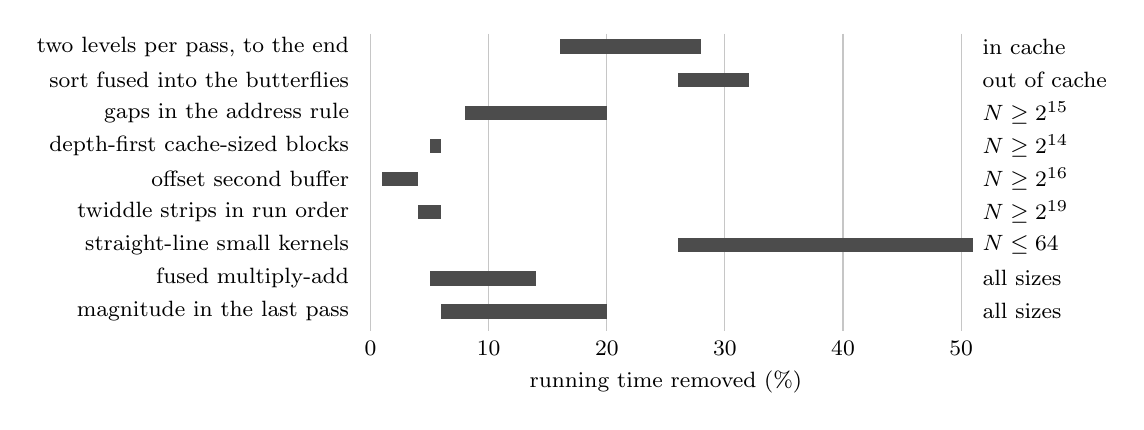
\begin{tikzpicture}[x=0.15cm,y=0.42cm,font=\footnotesize]
\foreach \v in {0,10,20,30,40,50} {
  \draw[gray!45] (\v,0.4) -- (\v,-8.6);
  \node[below] at (\v,-8.6) {\v};
}
\node[below] at (25,-9.5) {running time removed (\%)};
\def\bar#1#2#3#4#5{%
  \fill[black!70] (#2,-#1+0.22) rectangle (#3,-#1-0.22);
  \node[anchor=west] at (51,-#1+0.0) {#5};
  \node[anchor=east] at (-1,-#1) {#4};
}
\bar{0}{16}{28}{two levels per pass, to the end}{in cache}
\bar{1}{26}{32}{sort fused into the butterflies}{out of cache}
\bar{2}{8}{20}{gaps in the address rule}{$N\ge2^{15}$}
\bar{3}{5}{6}{depth-first cache-sized blocks}{$N\ge2^{14}$}
\bar{4}{1}{4}{offset second buffer}{$N\ge2^{16}$}
\bar{5}{4}{6}{twiddle strips in run order}{$N\ge2^{19}$}
\bar{6}{26}{51}{straight-line small kernels}{$N\le64$}
\bar{7}{5}{14}{fused multiply-add}{all sizes}
\bar{8}{6}{20}{magnitude in the last pass}{all sizes}
\end{tikzpicture}
\caption{Share of running time removed by each ingredient, as a range over the sizes where it applies. Double precision, two-lane vectors, Apple M4. Each bar compares the transform with and without that one ingredient; the first compares against a split walk whose last three levels run singly; the last against the transform followed by a magnitude loop.}
\label{fig:gains}
\end{figure*}

\section{Two Arithmetic Modes}\label{sec:modes}

A fused multiply-add is a single, exactly specified operation, and the two forms $a+b\,c$ and $a-b\,c$ map to one instruction on both of the architectures we build for.
What varies between builds is not the instruction but whether a compiler chooses to use it.
We remove that choice: contraction is disabled everywhere, and every fused operation is written explicitly, in one of those two forms only.
The transform then exists in two modes from one source.
\begin{itemize}
\item \emph{Fused.} Every multiply-add in the cells is one fused operation. It requires a fused multiply-add instruction at the tier in use.
\item \emph{Exact.} No fused operation appears anywhere. It is the mode for targets without the instruction and the reference for reproducibility.
\end{itemize}
Within a mode every vector width computes, lane by lane, the expression the scalar code computes, in the same order, from the same table.
Each mode therefore produces identical output on every target, vector width and compiler that implements it; the two modes differ from each other in the last bits, as they must.
The inverse undoes each pass exactly, with the halvings folded into its cells, so the inverse of the forward transform is the input with no normalisation pass.

\section{Magnitude Inside the Last Pass}\label{sec:mag}

Many consumers want $|X_k|$ and nothing else.
Just before the last pass's second shuffle layer, the real parts of a row's bins sit in one vector and the imaginary parts in another.
The magnitude output takes $\sqrt{\re^2+\im^2}$ there and stores each lane to its bin.
It omits the interleave, and it replaces the caller's own pass over the spectrum, which would have had to undo that interleave before it could vectorise.

\section{What Each Part Contributes}

Fig.~\ref{fig:gains} shows the share of running time that each ingredient removes, as the range observed across the sizes where it applies.
The figures are for double precision on one machine and are meant to show relative weight, not to rank libraries.
Two readings matter.
First, in cache the timing of the sort is neutral: with two doubles per vector a scattered store of one bin is a whole-vector store.
The fused sort pays when the transform leaves the cache, and by the lane argument it should pay earlier as vectors widen.
Second, the largest in-cache gain is the plainest: two levels per pass at every level, including the last.


\section{Against FFTW}

Table~\ref{tab:fftw} summarises running time against FFTW~3 with patient plans.
Each entry is the geometric mean, over the power-of-two sizes in the band, of this transform's time divided by FFTW's, with the smallest and largest ratio in parentheses; a value below one is faster.
The figures are estimates from one machine and one build of each library, not a ranking: an Apple M4, double precision, our fused mode on two-lane vectors, and FFTW as packaged for that machine.
FFTW plans were made with \texttt{FFTW\_PATIENT} up to $N=65536$ and \texttt{FFTW\_MEASURE} above; its inverse was planned to preserve its input, as ours does, and is unnormalised where ours is exact.
The magnitude row compares our magnitude output with FFTW's forward transform followed by a loop over its bins.

\begin{table}[b]
\caption{Running time relative to FFTW (geometric mean and range).}
\label{tab:fftw}
\centering
\begin{tabular}{@{}lcc@{}}
\toprule
Sizes & Forward & Inverse\\
\midrule
$16$ to $128$ & 0.67 (0.59--0.83) & 0.81 (0.70--1.00)\\
$256$ to $8192$ & 0.82 (0.76--0.92) & 0.73 (0.69--0.77)\\
$16384$ to $2^{20}$ & 0.77 (0.68--0.90) & 0.70 (0.64--0.76)\\
all, $16$ to $2^{20}$ & 0.76 (0.59--0.92) & 0.73 (0.64--1.00)\\
\midrule
magnitude, $16$ to $128$ & \multicolumn{2}{c}{0.61 (0.56--0.64)}\\
\bottomrule
\end{tabular}
\end{table}

Over all seventeen sizes the forward transform takes about three quarters of FFTW's time and the inverse a little less.
The forward lead is largest where the straight-line kernels apply and narrowest near $N=8192$ and $16384$, where the working set is the size of the first-level cache.

\section{Cumulative Error}

Every cell is a rotation followed by a sum and a difference, so a stage multiplies the norm by exactly $\sqrt2$ and no intermediate value exceeds the bound on the output; the inverse halves where the forward doubles.
There is no scaling pass in which rounding could collect, and nothing in the arithmetic depends on the size of the numbers.
We checked this by feeding a signal through the forward and inverse transforms repeatedly, each round taking the last round's output, at amplitudes of $1$, $10^{300}$ and $10^{-300}$ in double precision and $1$, $10^{30}$ and $10^{-30}$ in single.
After ten thousand rounds every result was finite and the largest relative deviation from the original was the same at all three amplitudes: of order $10^{-15}$ at $N=64$ and $2\times10^{-12}$ to $3\times10^{-12}$ at $N=1024$ and $4096$ in double precision, that is, a few units of $10^{-16}$ per round.
FFTW and the kernels of~\cite{obr} drift at the same rate under the same test.
One caution applies to the magnitude output: it forms $\re^2+\im^2$ directly, so it is limited to bins whose squares are representable.

\section{Relation to Prior Work}

The real rotation cell and the residue view of the split are Bruun's~\cite{bruun}; the normalized basis, the constant-along-a-run form of the rotation and the family of walks over one factor tree are from~\cite{obr}, on which this transform is built.
Fusing the bit-reversal into the butterfly stages of an in-place complex transform is due to Temperton~\cite{temperton}, and was developed for vector machines by Hegland~\cite{hegland,hegland2}; the shells and their exchange are that idea in the address-ledger language used here.
The autosort form attributed to Stockham~\cite{stockham} and the four-step method~\cite{bailey} are other schedules of the same exchanges.
Code generation for small transforms, and the planning of large ones, follow the practice established by FFTW~\cite{fftw}.
What we have set out is a particular combination: the exchanges placed in the second half so that every twiddle stays one per run; the conjugate-address real storage that keeps real and imaginary parts as separate runs to the last pass; the gapped address rule; and the two bit-reproducible arithmetic modes fed by an exactly reduced half-turn sine and cosine.

\section*{Acknowledgment}
This work was carried out with Fable, Astra, Sydney and Opus.

\begin{thebibliography}{99}
\bibitem{obr} J.~Rainstar, ``On Bruun, revisited,'' Malkuth Software, 2026.
\bibitem{bruun} G.~Bruun, ``$z$-transform DFT filters and FFT's,'' \emph{IEEE Trans. Acoust., Speech, Signal Process.}, vol.~26, no.~1, pp.~56--63, 1978.
\bibitem{ieee754} \emph{IEEE Standard for Floating-Point Arithmetic}, IEEE Std 754-2008, 2008.
\bibitem{tang} P.~T.~P. Tang, ``Table-lookup algorithms for elementary functions and their error analysis,'' in \emph{Proc. 10th IEEE Symp. Computer Arithmetic}, 1991, pp.~232--236.
\bibitem{sterbenz} P.~H. Sterbenz, \emph{Floating-Point Computation}. Englewood Cliffs, NJ: Prentice-Hall, 1974.
\bibitem{dekker} T.~J. Dekker, ``A floating-point technique for extending the available precision,'' \emph{Numer. Math.}, vol.~18, pp.~224--242, 1971.
\bibitem{temperton} C.~Temperton, ``Self-sorting in-place fast Fourier transforms,'' \emph{SIAM J. Sci. Stat. Comput.}, vol.~12, no.~4, pp.~808--823, 1991.
\bibitem{hegland} M.~Hegland, ``A self-sorting in-place fast Fourier transform algorithm suitable for vector and parallel processing,'' \emph{Numer. Math.}, vol.~68, pp.~507--547, 1994.
\bibitem{hegland2} M.~Hegland, ``Real and complex fast Fourier transforms on the Fujitsu VPP~500,'' \emph{Parallel Comput.}, vol.~22, pp.~539--553, 1996.
\bibitem{stockham} W.~T. Cochran \emph{et al.}, ``What is the fast Fourier transform?'' \emph{Proc. IEEE}, vol.~55, no.~10, pp.~1664--1674, 1967.
\bibitem{bailey} D.~H. Bailey, ``FFTs in external or hierarchical memory,'' \emph{J. Supercomput.}, vol.~4, pp.~23--35, 1990.
\bibitem{fftw} M.~Frigo and S.~G. Johnson, ``The design and implementation of FFTW3,'' \emph{Proc. IEEE}, vol.~93, no.~2, pp.~216--231, 2005.
\end{thebibliography}

\end{document}
